\documentclass{article}
\usepackage[dutch]{babel}
\usepackage[official]{eurosym}
\usepackage{graphicx}
\usepackage{epic,eepic}
\usepackage{mathtools}
\usepackage{caption}
\usepackage{float}
\usepackage{hyperref}
\usepackage{textcomp}
\setcounter{secnumdepth}{3}
\graphicspath{{fig/}}

\makeatletter
\renewcommand\subsubsection{%
   \@startsection{paragraph}{4}{0mm}%
      {-\baselineskip}%
      {.5\baselineskip}%
      {\normalfont\normalsize\bfseries}}
\makeatother

\title{Software Design Descriptions voor Schedule-Generator}
\author{Matthias Caenepeel \and Adam Cooman \and Alexander De Cock \and Zjef Van de Poel}
\date{20 mei 2011 Versie 3.0} 

\begin{document}

\maketitle

\newpage

% \newpage
% Signature page

% \newpage

\section*{Aanpassingsgeschiedenis}
\begin{itemize}
\item[.] 23/2/2011 versie 0.1: Aanmaak document 
\item[.] 27/2/2011 versie 0.2: Toevoeging delen over interfaces 
\item[.] 28/2/2011 versie 0.3: Toevoeging hoofdstuk over algoritme en Logical
\item[.] 28/2/2011 versie 1.0: Verbeteringen doorgevoerd 
\item[.] 17/3/2011 versie 1.1: Opmerkingen opdrachtgever in acht genomen en nodige aanpassingen gedaan. Gebruik van de GET en POST methode in de Site - Servlet interface grondiger uitgelegd 
\item[.] 28/3/2011 versie 2.0: Volledige revisie van het document en aanpassingen/toevoegingen doorgevoerd waar nodig.
\item[.] 20/5/2011 versie 3.0: Volledige revisie van het document. Toevoegine van nieuw algoritme, toevoeging van uitleg over de werking van de servlets op de server, toevoeging van nieuwe klassediagrammas.
\end{itemize}

%\section*{Preface}

\newpage
\tableofcontents

\newpage

%\section{Identified stakeholders and design concerns}

\section{Compositie}

\subsection{Design concerns}
Het doel van dit ontwerpstandpunt bestaat er in alle componenten van het systeem te identificeren, hun attributen te kenmerken en hun onderlinge verbanden te beschrijven. Deze beschrijving zal gebeuren aan de hand van een \textit{component diagram} en het \textit{deployment diagram}. Beide  zijn een onderdeel van de UML 2.0 modelleertaal.  

\subsection{Deployment Diagram}

Een deployement diagram geeft weer op welke manier de hard- en software wordt geconfigureerd tijdens de normale werking van het systeem. Hieronder volgt een beschrijving van de belangrijkste componenten in het diagram. 

\begin{figure}[H]%
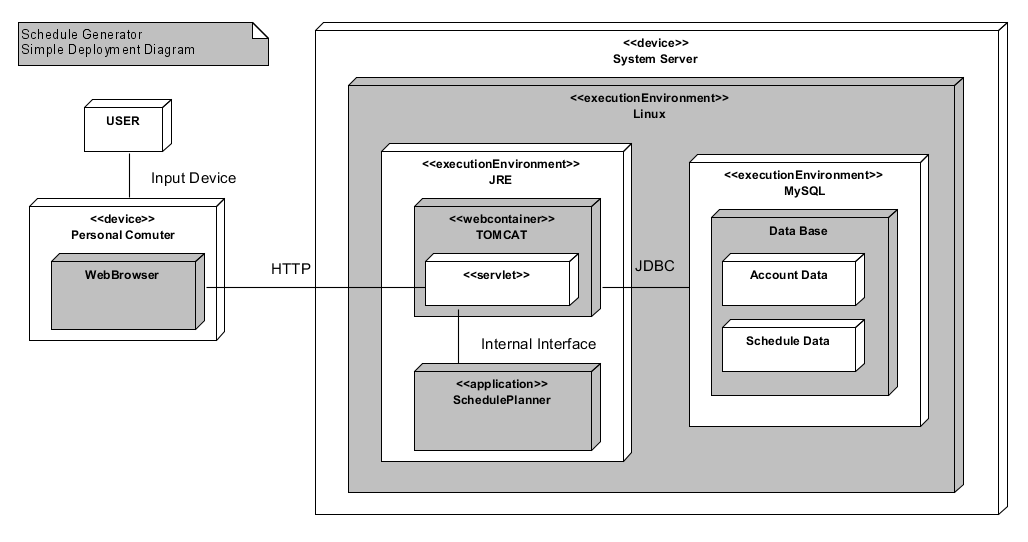
\includegraphics[width=\columnwidth]{DeploymentDiagram.png}%
\caption{Deployment Diagram}%
\end{figure}

\begin{description}

\item[Gebruiker] Een gebruiker die beschikt over een account kan zich aanmelden op de website via zijn gebruikersnaam en wachtwoord. Vervolgens zal hij beschikken over de functionaliteiten, eigen aan zijn gebruikertype. Als de gebruiker geen account heeft kan hij de site betreden als gast. Er wordt dan geen gebruikersgebonden informatie bijgehouden. Meer informatie over de verschillende gebruikertypes en functionaliteiten is voorzien in het SRS. \\
 
\item[Persoonlijke Computer] Toestel dat de hard- en software aan de gebruikerszijde bevat. Er worden geen onderstellingen gemaakt over de eigenschappen van dit toestel met uitzondering dat het instaat is een webbrowser te draaien met eigenschappen gelijkaardig aan die van Internet Explorer, Google Chrome of FireFox.  \\
 
\item[Webbrowser] Er worden geen specifieke onderstelling gemaakt met uitzondering van de reeds vermelde. \\
 
\item[Systeemserver] Tijdens de ontwikkeling van het project wordt Wilma als systeemserver gebruikt. De specificaties van de server worden volledig bepaald door de opdrachtgever en kunnen terug gevonden worden op \\ http://wilma.vub.ac.be/. \\
 
\item[Tomcat] Dit is een webcontainer ontwikkeld door Apache die onder andere toelaat servlets te draaien op een Linux server. Deze servlets zullen de vragen van de gebruiker opvangen en op dynamische wijze webinhoud generen als antwoord. Deze webinhoud zal hoofdzakelijk worden beschreven via XHTML en CVS. Voor meer informatie over Tomcat kan men terecht op \\ http://tomcat.apache.org/. \\
 
\item[Database] De database  maakt onderdeel van de hardware van de systeemserver en bevat zowel de account informatie als de informatie die relevant is voor het opstellen van de lessenroosters. Om gegevens uit de database toegankelijk te maken voor elementen uit de Java runtime environment (JRE) zal gebruikt worden gemaakt van JDBC. Dit is een Java Application Programming Interface ontwikkeld door Sun. Een overzicht wordt gegeven op \\ www.oracle.com/technetwork/java/javase/tech/index-jsp-136101.html \\

\end{description}


%\subsection{Component Diagram}

%Zal later worden toegevoegd




%------------------------------------------------------------------------------------------------------------------------------------------------------------------


\section{Interfaces}
% HTTP
% Adam schrijft dit het is toegelaten dat je zelf de punten een beke invult

% HTML bestand met javascript om tabs te maken
% HTML bestand met CSS voor layout
% Javascript met CSS intern voor tabber
% HTML met server via HTTP (GET en POST)
% Servlet via interface van Zjef en MySQL met Database

\subsection{Design concerns, algemeen}

\begin{figure}[H]
\unitlength=0.3\textwidth
\begin{center}
\begin{picture}(3,1)
%serverlijnen
\put(0.2,0.2){Server}
\put(0.0,0.0){\line(1,0){1.6}}
\put(0.0,0.0){\line(0,1){1.0}}
\put(1.6,0.0){\line(0,1){1.0}}
\put(0.0,1.0){\line(1,0){1.6}}
%browser
\put(2.4,0.2){Browser}
\put(2.2,0.0){\line(1,0){1.6}}
\put(2.2,0.0){\line(0,1){1.0}}
\put(3.8,0.0){\line(0,1){1.0}}
\put(2.2,1.0){\line(1,0){1.6}}
%XHTML
\put(2.32,0.7){Webpagina}
\put(2.4,0.5){XHTML}
\put(2.3,0.9){\line(1,0){0.5}}
\put(2.8,0.4){\line(0,1){0.5}}
\put(2.3,0.4){\line(0,1){0.5}}
\put(2.3,0.4){\line(1,0){0.5}}
%CSS
\put(3.0,0.7){Stylesheet; CSS}
\put(2.95,0.8){\line(1,0){0.8}}
\put(2.95,0.65){\line(0,1){0.15}}
\put(2.95,0.65){\line(1,0){0.8}}
\put(3.75,0.65){\line(0,1){0.15}}
% CSS naar XHTML
\put(2.82,0.725){\line(1,0){0.11}} 
%Javascript
\put(3.0,0.5){Script; Javascript}
\put(2.95,0.6){\line(1,0){0.8}}
\put(2.95,0.45){\line(0,1){0.15}}
\put(2.95,0.45){\line(1,0){0.8}}
\put(3.75,0.45){\line(0,1){0.15}}
% Javascript naar XHTML
\put(2.82,0.525){\line(1,0){0.11}} 
%database
\put(0.15,0.6){Database}
\put(0.1,0.9){\line(1,0){0.5}}
\put(0.6,0.4){\line(0,1){0.5}}
\put(0.1,0.4){\line(0,1){0.5}}
\put(0.1,0.4){\line(1,0){0.5}}
%servlet
\put(1.1,0.8){Servlet}
\put(1.1,0.6){JAVA}
\put(1.0,0.95){\line(1,0){0.5}}
\put(1.5,0.55){\line(0,1){0.4}}
\put(1.0,0.55){\line(0,1){0.4}}
\put(1.0,0.55){\line(1,0){0.5}}
% Files
\put(1.1,0.25){Files}
\put(1.1,0.1){XML}
\put(1.0,0.4){\line(1,0){0.5}}
\put(1.5,0.05){\line(0,1){0.35}}
\put(1.0,0.05){\line(0,1){0.35}}
\put(1.0,0.05){\line(1,0){0.5}}
% lijn Files naar Servlets
\put(1.25,0.42){\line(0,1){0.11}} 
%lijn MySQL
\put(0.65,0.7){MySQL}
\put(0.62,0.65){\line(1,0){0.36}}
%lijn HTTP
\put(1.8,0.7){HTTP}
\put(1.52,0.65){\line(1,0){0.76}}
\end{picture}\\[3mm]
\caption{Overzicht van de verschillende delen van het programma}
\end{center}
\end{figure}

In de structuur van ons programma bestaan verschillende elementen met verschillende taken. Deze moeten met elkaar interageren volgens het bovenstaande schema. De lijnen tussen de verschillende blokken noemen we interfaces en zullen in het volgende deel van het Software Design Document besproken worden. Vooraleer daarmee te beginnen een kort overzicht van de taken die elk blok uit het diagramma uitvoert.

\begin{description}
  \item[Webpagina, XHTML] \hfill \\
  In het XHTML bestand wordt de inhoud van de webpagina geplaatst. 
  \item[Stylesheet, CSS] \hfill \\
  In het stylesheet wordt de lay-out van de webpagina beschreven.
  \item[Script, Javascript] \hfill \\
  In het script word beschreven wanneer welk deel van de webpagina weergegeven wordt. We gebruiken tabbladen om de functionaliteiten die een gebruiker krijgt duidelijk weer te geven. Ht beheer van die tabbladen gebeurt met het javascript "tabber" dat ontwikkeld werd door derden;
  \item[Servlet, JAVA] \hfill\\
  De servlets runnen op tomcat en genereren de XHTML code, afhankelijk van de eigenschappen van de gebruiker.
  \item[Database] \hfill\\
  In de database wordt de informatie van gebruikers en de kalender opgeslaan.
  \item[Files] \hfill\\
  De files bevatten wijzigbare parameters van het programma. Ze zijn in een XML bestand opgeslaan.
\end{description}

Het schema is geen volledig correcte weergave van de werkelijkheid omdat het stylesheet en het script zich ook op de server bevinden en door de browser opgehaald worden van de server via een HTTP protocol. Om volledig correct te zijn zouden die twee onderdelen van het schema zich dus ook op de server moeten bevinden. Om alles overzichtelijk te houden heeft de auteur beslist om ze bij de browser te plaatsen, omdat de browser het ophalen van de server voorziet en niet de gebruiker.

\subsection{Interface:  XHTML - CSS voor Layout}
\subsubsection{Initialiseren} 

Om het .css bestand aan de XHTML pagina te linken moet in de header van de XHTML code het volgende voorzien worden
\begin{verbatim}
<link rel="stylesheet" href="style.css" type="text/css"> 
\end{verbatim}
Hierin zijn de volgende elementen te herkennen:
\begin{itemize}
\item[] \texttt{rel="stylesheet"}: Duidelijk maken dat de link een link naar een stylesheet is. Deze tag verandert niet \\[-5mm]
\item[] \texttt{type="text/css"}: Duidelijk maken dat de stylesheet in css code geschreven is. Deze tag verandert ook niet \\[-5mm]
\item[] \texttt{href="style.css"}: De naam van het css bestand. Als die zich op een andere locatie bevindt dan de XHTML pagina moet het pad naar die map hierin toegevoegd worden \\[-5mm]
\end{itemize}

\subsubsection{Gebruiken} 

In de XHTML code moet niet veel toegevoegd worden om de css op te roepen, enkel een id tag op de volgende manier om onderscheid te maken tussen verschillende gedefini\"{e}erde stijlen in de css code. Als voorbeeld wordt het toevoegen van een id aan een rij van een tabel gegeven om aan te tonen hoe dit moet.
\begin{verbatim}
<tr id="MainBottom">
\end{verbatim}
De naam van het id staat tussen de aanhalingstekens.\\

In het CSS bestand kan de code voor de stijl van hetzelfde id geschreven worden door gebruik te maken van hekje. Als voorbeeld de CSS code die de stijl beschrijfd van de tabelrij uit het vorige voorbeeld.
\begin{verbatim}
tr#MainBottom {
	height:300px;
}
\end{verbatim}

\subsection{Interface: XHTML - Javascript voor tabbladen}
\subsubsection{Initialiseren} 

Het oproepen van het javascript bestand gebeurt in de header van het XHTML bestand dat de inhoud van de site beschrijft met de volgende code.
\begin{verbatim}
<script type="text/javascript" src="tabber-minimized.js"></script>
\end{verbatim}
Hierin zijn de volgende elementen te herkennen:
\begin{itemize}
\item[] \texttt{type="text/javascript"}: Duidelijk maken dat het javascript is. Deze tag verandert niet \\[-5mm]
\item[] \texttt{src="tabber-minimized.js"}: De naam van het javascript bestand. Als die zich op een andere locatie bevindt dan de HTML pagina moet het pad naar die map hierin toegevoegd worden \\[-5mm]
\end{itemize}

\subsubsection{Gebruiken}
Om dan een tabblad aan te maken en er inhoud in te plaatsen wordt gebruik gemaakt van div elementen in de XHTML code. dit gebeurd op de volgende manier:
\begin{verbatim}
<div class="tabber">
<div class="tabbertab" title="Tabblad 1">
Inhoud van het eerste tabblad
</div>
<div class="tabbertab" title="Tabblad 2">
Inhoud van het tweede tabblad
</div>
</div>
\end{verbatim}
In de buitenste div staat het volgenden:
\begin{itemize}
\item[]  \texttt{class="tabber"}: dit vertelt aan het javascript dat er tabbladen volgen. Het laat toe om geneste tabbladen te gebruiken \\[-5mm]
\end{itemize}
In de binnenste divs, \'{e}\'{e}n per tabblad:
\begin{itemize}
\item[] \texttt{class="tabbertab"}: dit vertelt aan het javascript dat er tabbladen volgen. Het laat toe om geneste tabbladen te gebruiken \\[-5mm]
\item[] \texttt{title="Tabblad 1"}: In het title tag staat de titel van het tabblad die bovenaan weergegeven wordt \\[-5mm]
\end{itemize}

\subsection{Interface: Javascript - CSS voor tabbladen}

Het Javascript tabber dat gebruikt wordt bevat interne links naar het CSS bestand. De exacte werking van de interface is niet gekend omdat tabber een programma is dat geschreven is door derden. De nodige css code werd aan het stijlbestand toegevoegd zodat alles werk. Het is nu mogelijk om de layout van de tabbladen te defini\"{e}ren in het stijlbestand. De nodige onderverdelingen die toegevoegd moeten worden zijn de volgende:

\begin{verbatim}
.tabberlive .tabbertabhide {}
.tabber {}
.tabberlive {}
ul.tabbernav{}
ul.tabbernav li {}
ul.tabbernav li a {}
ul.tabbernav li a:link {}
ul.tabbernav li a:visited {}
ul.tabbernav li a:hover{}
ul.tabbernav li.tabberactive a{}
ul.tabbernav li.tabberactive a:hover{}
.tabberlive .tabbertab {}
\end{verbatim}


\subsection{Interface: Browser - Server: HTTP}

\subsubsection{Concerns}
Omdat de algemene kalender en andere gegevens in een database op de server zullen opgeslaan zijn en omdat de gebruiker vanop zijn computer thuis via de website die informatie te zien moet krijgen, moet er een communicatie tussen de server en de browser van de gebruiker zijn. Zoals bij de meeste websites werd gekozen om het het HTTP protocol te werken. We laten niet toe dat de gebruikers rechtstreeks met de database communiceren om te vermijden dat ze informatie te zien krijgen die ze niet mogen zien, en om de informatie op een overzichtelijke manier te structureren. Daarom werken we met Servlets die op server runnen en die de besproken taken verrichten. De volgende paragrafen beschrijven dus de communicatie tussen de browser van de gebruiker en de servlets.

\subsubsection{Attributes}

Uit het HTTP protocol zullen de GET en POST functies gebruikt worden door onze toepassing. Een HTTP pakket bestaat uit twee delen, de \textit{header} en de \textit{body}.
\begin{description}
\item[GET] Deze methode vraagt een bepaalde pagina aan de server en zet alles in de \textit{header}. Het is de methode die gebruikt wordt bij het klikken op een link van een site. Deze zal dus de meest gebruikte methode zijn om te communiceren met de server. \\
\item[POST] Deze methode stuurt informatie door in de \textit{body} van het paket.\\
\end{description}
De manier waarop de informatie doorgestuurd zal worden hangt af van de plaats. Gevoelige informatie, zoals wachtwoorden zal via een POST verzonden worden, omdat de header gemakkelijk zichtbaar is voor gebruikers. Lange informatie, zoals beschrijvingen van vakken zal ook via de POST methode verzonden worden, omdat de lengte van de \textit{header} beperkt is. \\

Andere informatie, zoals het opvragen van het lessenrooster zal via de GET methode gebeuren. De waarden van de zoekactie worden dan in de link geplaatst door een script dat nog ontwikkeld moet worden en waarvan de interface met de XHTML pagina gelijkenissen zal vertonen met die voor de tabbladen. \\

\subsubsection{GET}

We gebruiken HttpServlets die de doGet methode bevatten om een Get aanvraag binnen te krijgen en die te beantwoorden. Beschouw als voorbeeld de volgende servlet. Hij stuurt het antwoord Hallo terug naar de gebruiker als die de juiste URL ingegeven heeft. Welke URL dat is wordt beschreven in een XML bestand dat zich op de server bevindt en een bepaalde URL aan een Servlet koppelt.

\begin{verbatim}
public class test2 extends HttpServlet {
public void doGet(HttpServletRequest request,
                  HttpServletResponse response)
  throws ServletException, IOException {
    response.setContentType("text/html");
    PrintWriter out = response.getWriter();
    out.println("Hallo");
  }
}	
\end{verbatim}

Om variabelen mee te geven naar de servlet met de GET methode wordt gerbuik gemaakt van een vraagteken. Als een variabele \textit{ID} meegegeven wordt aan een URL gebeurt dit op de volgende manier:
\begin{verbatim}
servletnaam?ID=waarde
\end{verbatim}

in de doGet methode kan de waarde van de variabele opgeroepen worden met de getParameter methode:
\begin{verbatim}
String ID = request.getParameter("ID");
\end{verbatim}


\subsubsection{POST}
Bij het gebruik van een GET om variabelen aan de servlet door te geven staan de variabelen en hun waarden allemaal in de URL. Voor gevoelige informatie zoals wachtwoorden, of als er zeer veel informatie doorgegeven moet worden (de maximum lengte van een URL in internet explorer is 2083 tekens) is deze methode niet geschikt. Daarvoor zal de POST methode gebruikt worden.\\

Er zal dus enkel gebruik gemaakt worden van de POST methode bij het verzenden van een HTML Form. Deze HTML structuur bevat velden die ingevuld kunnen worden door de gebruiker en een knop waar de gebruiker op moet klikken om de informatie door te sturen. Om een variabele PASS door te sturen met een POST naar de servlet zou de code voor de form er als volgt uitzien:
\begin{verbatim}
<FORM METHOD="POST" ACTION="servlet">
<P> 
<INPUT TYPE="PASSWORD" NAME="PASS"><BR>
<INPUT TYPE="submit" VALUE="Send">
</P>
</FORM>
\end{verbatim}
In de begintag van het form wordt de opstuurmethode gedefinieerd in het METHOD attribuut. deze kan de waarden POST en GET aannemen. In het ACTION attribuut wordt de locatie van de servlet waar de form naartoe gestuurd wordt gespecifieerd.\\
Het inputveld waar de gebruiker de data moet invoeren wordt gemaakt met een INPUT tag. Het attribuut NAME definieert de naam van de variabele en het attribuut TYPE definieert de vorm van het invoerveld\footnote{dit kan veel verschillende vormen aannemen, zie \href{http://www.w3.org/TR/html401/interact/forms.html}{www.w3.org}}.\\
Als laatste essentieel deel van de Form is er de knop waar de gebruiker moet op klikken om de gegevens door te sturen. Dit is opnieuw een INPUT tag, maar nu van het type submit. in het Value attribuut staat de tekst die op de knop moet weergegeven worden.\\

In de servlet kan de doPost methode geimplementeerd worden om de verschillende forms te verwerken. Opnieuw kunnen de variabelen opgevraagd worden met de getParameter methode:
\begin{verbatim}
String ID = request.getParameter("PASS");
\end{verbatim}

Om meer variabelen mee te sturen met een form, is het mogelijk om onzichtbare INPUT tags te defini\"{e}ren in het HTML Form. daarmee kan aan de Servlet bijvoorbeeld meegegeven worden welk Form ingevuld is. 


\subsection{Interface: Database interface}

\subsubsection{Concerns}
De interface met de MySQL database wordt geleverd door de reeds bestaande java library MySQL Connector/J1 \footnote{http://dev.mysql.com/downloads/connector/j/}.
Deze biedt de mogelijkheid om queries uit te voeren vanuit Java code en de resultaten van deze query uit te lezen.

Om eenvoudig en flexibel te kunnen werken met de database vanuit de object geori�nteerde code is er een extra interface geschreven rond de MySQL Connector.
Deze levert op een eenvoudig te implementeren manier de mogelijkheid om rechtstreeks Java objecten op te slaan en deze ook dusdanig als objecten uit te lezen, met inbegrip van alle onderlinge verbanden tussen de objecten.

\subsubsection{design}

\begin{figure}[H]%
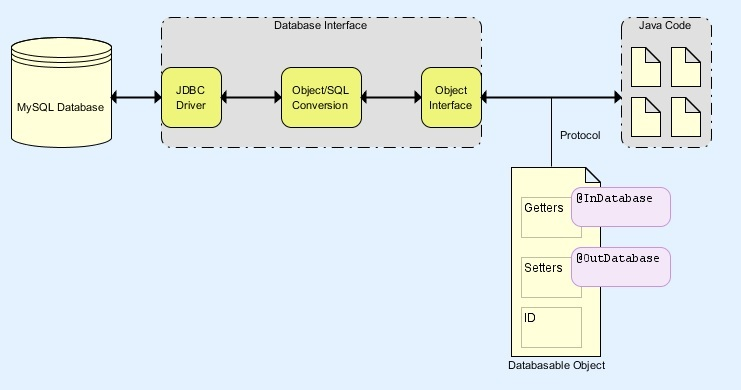
\includegraphics[width=\columnwidth]{DATA1.jpg}%
\caption{Overzicht}%
\end{figure}

\begin{figure}[H]%
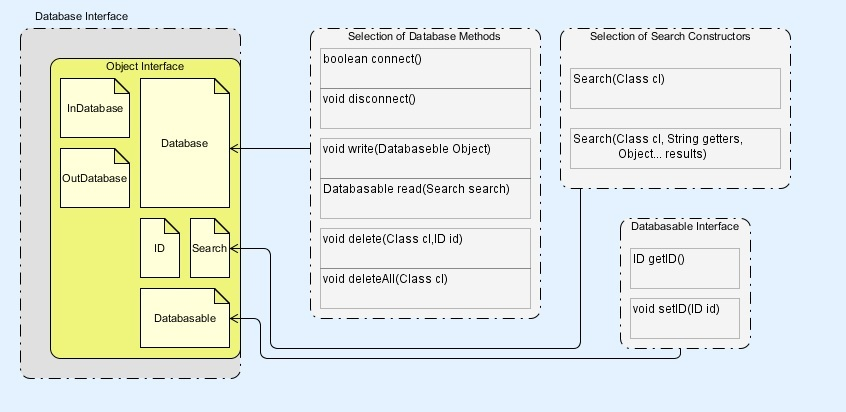
\includegraphics[width=\columnwidth]{DATA2.jpg}%
\caption{Overzicht van belangrijkste klasses en methodes}%
\end{figure}

De interface biedt communicatie met de database op basis van objecten die aangeboden of opgevraagd worden aan de interface. De interface zal dan zelf de nodige informatie extraheren vanuit het object om het in de database op te slaan, of zal de juiste informatie in het object steken om het uit de database te lezen.
Om deze data extractie correct te laten gebeuren, moet het object aan een bepaald protocol voldoen.
Dit protocol dient zich aan onder de vorm van de java interface klasse 'Databasable'.
Het object dient deze klasse te implementeren.

De getters en setters van de parameters die in en uit de database gehaald moeten worden, moeten worden aangeduid met een Annotation. De interface zal tijdens het vertalen via Reflection in Java zo de juiste methodes kunnen selecteren uit de klasse.
Meer bepaald:
\begin{itemize}
	\item[-] Getters annoteren met @InDatabase
	\item[-] Setters annoteren met @OutDatabase
\end{itemize}


Tijdens het wegschrijven van een object worden alle parameters die teruggegeven worden door de @InDatabase getters opgeslagen in de database.
Tijdens het uitlezen worden alle @OutDatabase setters opgeroepen met de waarde die uitgelezen werd uit de database.

Elk object krijgt een unieke ID (uniek binnen zijn klasse) wanneer hij naar de Database wordt geschreven. Hierdoor moet een parameter van de klasse 'ID' bijgehouden worden. 
De gebruiker dient deze slechts te voorzien  samen met de methodes van de interface Databasable; de invulling van deze ID gebeurt automatisch.

Door dit protocol wordt het schrijven van een object naar de database vereenvoudigd tot het schrijven van:
\begin{verbatim}
myDatabase.write(myObj);
\end{verbatim}

Het uitlezen gebeurt via een 'Search' object, waarmee een bepaald zoek criterium kan opgesteld worden:
\begin{verbatim}
myObj=myDatabase.read(mySearch);
\end{verbatim}

De interface zorgt er ook voor dat de links tussen verschillende objecten ook mee afgehandeld worden. Zie de voorbeelden voor meer detail.
Alle voorwaarden om de Databasable interface correct te implementeren zijn te vinden in de Javadoc commentaar van Databasable.

Voorbeelden van correcte implementatie zijn te vinden in de google-code repository bij:
trunk/Database/Voorbeeld

%\subsubsection{Elementen}
%
%\begin{itemize}
%\item[-] Database \\[-5mm]
%\begin{itemize}
%\item[-] \textbf{Database}: Handle naar de database. Levert methodes om tabellen in te lezen, opzoekingen te 		doen, objecten weg te schrijven en dergelijke.
%\item[-] \textbf{Table}: Een enkele tabel uit de database
%\item[-] \textbf{Element}: Een element van een tabel
%\end{itemize}		
%\item[-] Interface \\[-5mm]
%\begin{itemize}
%\item[-] \textbf{Databasable}: Inteface* die duidelijk maakt dat een object van een klasse die 	\textit{Databasable} implementeert, in de database geschreven, of uit de database gelezen 	kan worden. \\[-5mm]
%\item[-] \textbf{InDatabase}: Annotation* die duidelijk maakt dat een bepaalde parameter van een object in de 		database bewaard moet worden. \\[-5mm]
%\item[-] \textbf{OutDatabase}: Annotation* die duidelijk maakt dat een bepaalde parameter van een object  uit de 		database gelezen en naar het object gekopieerd moet worden. \\[-5mm]
%\end{itemize}		
%\end{itemize}		
%		
%*: Java terminologie

\subsection{Interface: XML interface}

\subsubsection{Concerns}

Er bestaan reeds talloze XML parsers, maar omwille van flexibiliteit en modificeerbaarheid is er een eigen parser geschreven.
Zo is het huidige format niet meer zuiver xml, maar zijn extra features toegevoegd die extra functionaliteiten toevoegen, maar op een manier dat 'echte' xml parsers de door deze parser gegenereerde xml nog steeds kan weergeven.

\subsubsection{Design}

Een boomstructuur van java objecten wordt opgesteld vanuit een xml bestand, of omgekeerd.
Uitgedrukt in BNF:
\begin{verbatim}
<XMLDocument> ::= {<XMLElement>}
<XMLElement> ::= <ElementWithValue> | <ElementWithChildren>
<ElementWithChildren> ::= <name><value>
<ElementWithChildren> ::= <name>{<XMLElement>}
<name> ::= {<any_character_no_space>}
<value> ::= {<any_character>}
\end{verbatim}

\begin{figure}[H]%
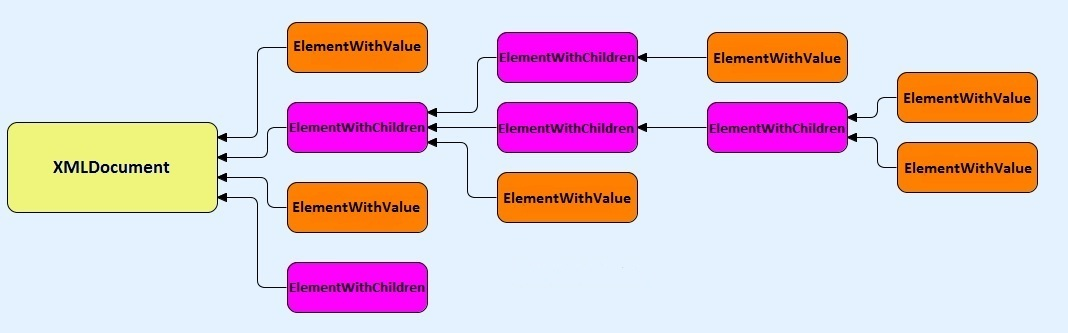
\includegraphics[width=\columnwidth]{XML1.jpg}%
\caption{Voorbeeld van XMLDocument}%
\end{figure}

\subsubsection{Features}
\textbf{Tags}
Specifieke tags kunnen toegevoegd worden aan de elementen:
\begin{verbatim}
<element tag=XXX> ... </element tag=XXX>
\end{verbatim}

\textbf{Code tag}
Door deze tag toe te voegen, wordt alle opmaak binnenin het element genegeerd. Dit kan gebruikt worden wanneer men bijvoorbeeld html code wil opslaan in een xml-element.
Normaal gezien zouden de html tags interfereren met de xml tags, maar de code-tag zorgt ervoor dat alles wat binnen de tags van het element staat gewoon als tekst aanzien wordt
\textbf{Link tag}
Deze tag laat toe om links te genereren tussen verschillende xml bestanden.
Links worden aangegeven door de link tag, waarna in de 'value' van het element een link kan worden toegevoegd tussen '� �'.  
Zie voorbeeld hieronder:

\begin{figure}[H]%
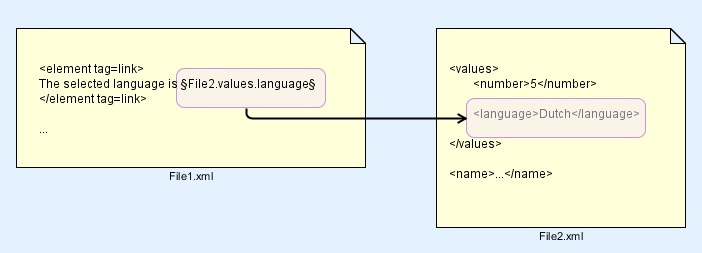
\includegraphics[width=\columnwidth]{XML2.jpg}%
\caption{Link tussen xml files}%
\end{figure}

Na het inladen van File1.xml heeft 'element' de waarde 'The selected language is Dutch'.

%\subsubsection{Elementen}
%
%\begin{itemize}
%\item[-] \textbf{XMLDocument}: Object verwijzende naar een XML bestand. Een XMLDocument bevat een lijst van 	XMLElement \\[-5mm]
%\item[-] \textbf{XMLElement}: Element van een XML bestand. Een element heeft een bepaalde waarde, of bevat zelf een 	aantal andere elementen. \\[-5mm]
%\begin{itemize}
%	\item[-] \textbf{ElementWithValue}: Element met een waarde \\[-5mm]
%	\item[-] \textbf{ElementWithChildren}: Element met lijst van andere elementen, zijn \textit{Children}.(\textit{Children} kunnen op hun beurt ook weer \textit{ElementWithChildren} of \textit{ElementWithValue} zijn) \\[-5mm]
%\end{itemize}		
%\item[-] \textbf{XMLParser}: Levert methodes om een XML bestand, gecre�erd met deze interface, weer in te laden naar 	een XMLDocument 
%\end{itemize}
%
%\subsubsection{Schema}
%
%\begin{figure}[H]
%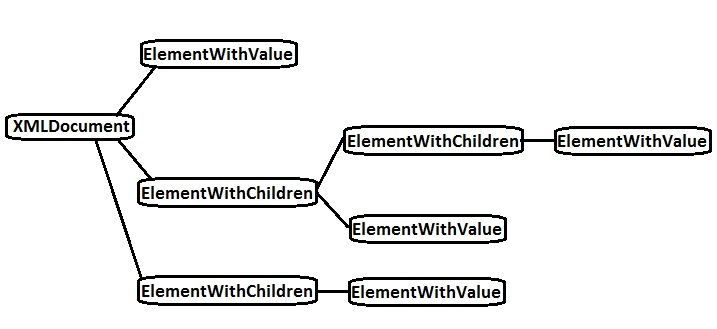
\includegraphics[width=\columnwidth]{XML.png}%
%\caption{Voorbeeld van een \textit{XMLDocument}}%
%\end{figure}

\newpage

%-----------------------------------------------------------------------------------------------------------------------------------------------------

\section{Logical}
\subsection{Design concerns}
Om de lessenrooster op te stellen en uit te lezen zijn er verschillende klasses nodig die alle verschillende participerende objecten voorstellen.

\subsection{Elementen}
\subsubsection{Entiteiten}

\begin{itemize}
	\item[-] Lessen structuur \\[-5mm]
	\begin{itemize}
	  \item[-] \textit{Course}: Les die gevolgd kan worden \\ [-5mm]
	  \item[-] \textit{Subcourse}: Onderdeel van een les; bv hoorcollege, labo of oefeningenles \\[-5mm]
	  \item[-] \textit{Program}: Verzameling van lessen die in een pakket zitten. Bijvoorbeeld 1e bachelor ingenieurswetenschappen \\[-5mm]
	\end{itemize}
	\item[-] Gebouwen strucuur \\[-5mm]
	\begin{itemize}
	  \item[-] \textit{Building}: Gebouw \\[-5mm]
    \item[-] \textit{Room}: Lokaal in een gebouw waar les gegeven kan worden \\[-5mm]
    \item[-] \textit{Hardware}: Materiaal beschikbaar in een lokaal \\[-5mm]
	\end{itemize}
	\item[-] Personen structuur \\[-5mm]
	\begin{itemize}
	  \item[-] \textit{Student}: Persoon die lessen kan volgen \\[-5mm]
    \item[-] \textit{Educator}: Persoon die lessen kan geven; zowel professoren, docenten en assistenten \\[-5mm]
	\end{itemize}
	\item[-] Andere \\[-5mm]
	\begin{itemize}
	  \item[-] \textit{Faculty}: Faculteit van de universiteit \\[-5mm]
	\end{itemize}
\end{itemize}

\subsubsection{Relaties}

\begin{itemize}
\item[-] Lessen structuur \\[-5mm]
	\begin{itemize}
	\item[] Elke \textit{Course} bestaat uit een of meerdere \textit{SubCourses} die in opgeteld het gehele vak weergeven. \\[-5mm]
	\item[] \textit{Courses} zelf worden gegroepeerd in een \textit{Program}. \\
	\end{itemize}
\item[-]Gebouwen structuur \\[-5mm]
\begin{itemize}
	\item[] Een gebouw beschikt over een lijst met \textit{Rooms}, die op zich een lijst met beschikbare \textit{Hardware} bijhoudt. \\[-5mm]
	\item[] Een gebouw kan ingedeeld worden onder een faculteit. \\[-5mm]
	\end{itemize}
\item[-] Personen \\[-5mm]
	\begin{itemize}
	\item[] Elke \textit{Student} is ingeschreven in een \textit{Program} en een lijst met afzonderlijke \textit{Courses} die ze volgen.  \\[-5mm]
	\item[] Een \textit{Educator} beschikt over een lijst \textit{Courses} en \textit{SubCourses} die ze geven. \\[-5mm]
\end{itemize}		
\end{itemize}

\subsubsection{UML Diagrammma}

\begin{figure}[H]%
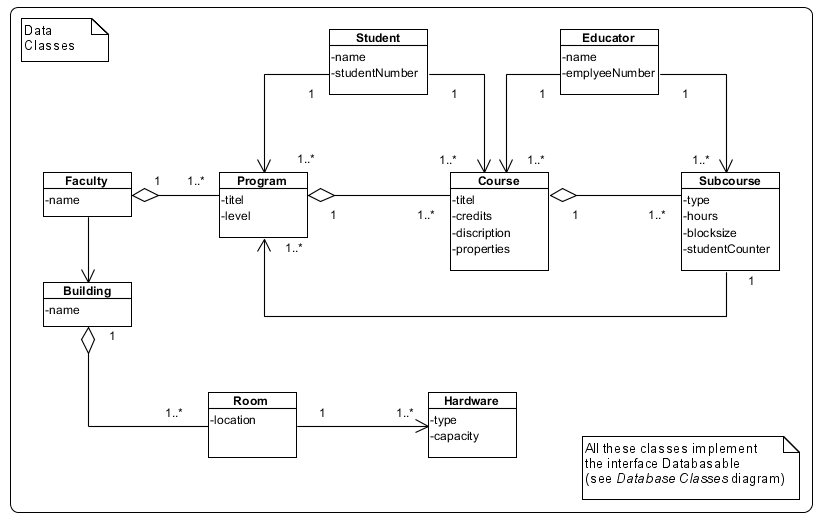
\includegraphics[width=\columnwidth]{UML_DataClasses.png}%
\caption{Dataclasses}%
\end{figure}

%\begin{figure}[H]%
%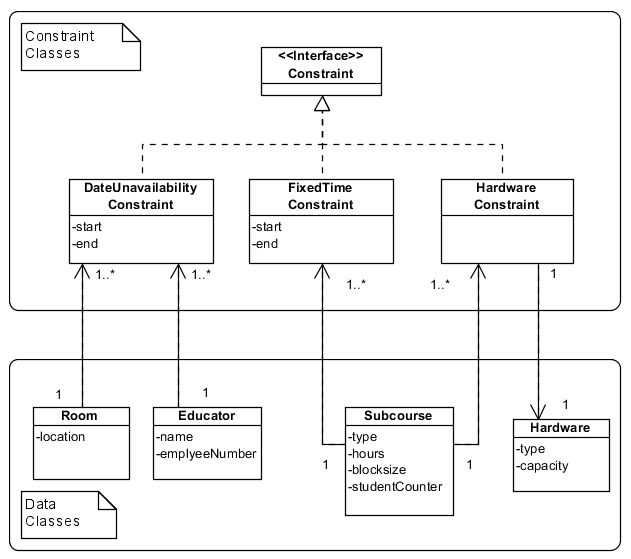
\includegraphics[width=\columnwidth]{UML_ConstraintClasses.png}%
%\caption{Constraint classes}%
%\end{figure}


\section{Website/Server Communicatie}

\subsection{Beknopte achtergrond informatie}

De webpagina�s worden op de server gegenereerd door een Java Servlet. Deze ontvangt de requests van de website.
De website is modulair opgebouwd door middel van tabbladen. Elk tabblad vervult een afgebakende functie (zoals het bekijken van de eigen kalender, het beheer van de cursussen voor de admins,�). De tabbladen die een gebruiker te zien krijgt is afhankelijk van zijn gebruikerstype.

\subsection{Inplementatie en Communicatie}

Om de benodigde modulariteit te implementeren bestaat er een aparte java klasse/object voor elke functionaliteit/tabblad. Deze ontvangen de request van de browser wanneer het tabblad zijn pagina opvraagt en genereren aan de hand hiervan een pagina als antwoord. Deze pagina bestaat uit een statisch deel, die uit een template file gelezen wordt. Het dynamische deel wordt aangevuld aan deze template. \\
Om de beveiliging te controleren (gebruikers die tabbladen opvragen waarvoor ze niet gemachtigd zijn) en om de site in verschillende talen te kunnen weergeven, is er een centraal punt nodig die deze taken, gemeenschappelijk aan alle functies, op zich neemt. \\
Hiervoor is er een centrale servlet, \textit{MainServlet}, opgesteld die alle request van de browser ontvangt. \\
De taken zelf worden uitgevoerd door \textit{PseudoServlets}. De MainServlet stuurt de binnengekregen request door naar de correcte PseudoServlet (\textit{public String processRequest(�)}), op basis van een tag in de query string. Doordat alle requests gebundeld worden door de MainServlet, kan deze op basis van de account nagaan of deze de gevraagde PseudoServlet toegankelijk is voor de gebruiker; zo niet kan deze de request tegenhouden en niet doorsturen naar de desbetreffende PseudoServlet. \\
De PseudoServlet krijgt via de methode processRequest(�)  de opdracht om een String te genereren die de html pagina voorstelt. Vooraleer deze String naar de browser wordt doorgestuurd door de MainServlet, zal deze eerst door een vertaler gestuurd worden, zodat elke gebruiker zijn eigen taal kan instellen, zonder dat elke PseudoServlet hier apart rekening mee moet houden. \\
Verder bestaan er ook \textit{PseudoServletsForApplets} (subklasse van PseudoServlet). Deze genereren via processRequest(�) een html pagina waarin een Java applet geladen wordt. De applet zelf kan communicatie aangaan met de PseudoServlet om meer informatie in te laden of om zelf informatie door te sturen onder de vorm van geserialiseerde Java objecten. Dit delegeert de MainServlet naar de PseudoServlet via processAppletRequest(�). \\
De generatie van de totale pagina gebeurt nu eenvoudig. De MainServlet krijgt een request binnen waarvan de �id� niet is ingesteld. Dit triggert de creatie van een login pagina. Na het inloggen krijgt de gebruiker een id toegewezen die hij met alle requests zal doorsturen ter identificatie (de id wordt gekoppeld aan een account aan de server zijde). Na het inloggen genereert de MainServlet een pagina waarvoor er voor elke PseudoServlet van de gebruiker een tabblad voorzien is.
In elk tabblad zit er een iframe waarbij de url naar de desbetreffende PseudoServlet verwijst. De webpagina zal nu alle correcte tabbladen kunnen inladen.

\begin{figure}%
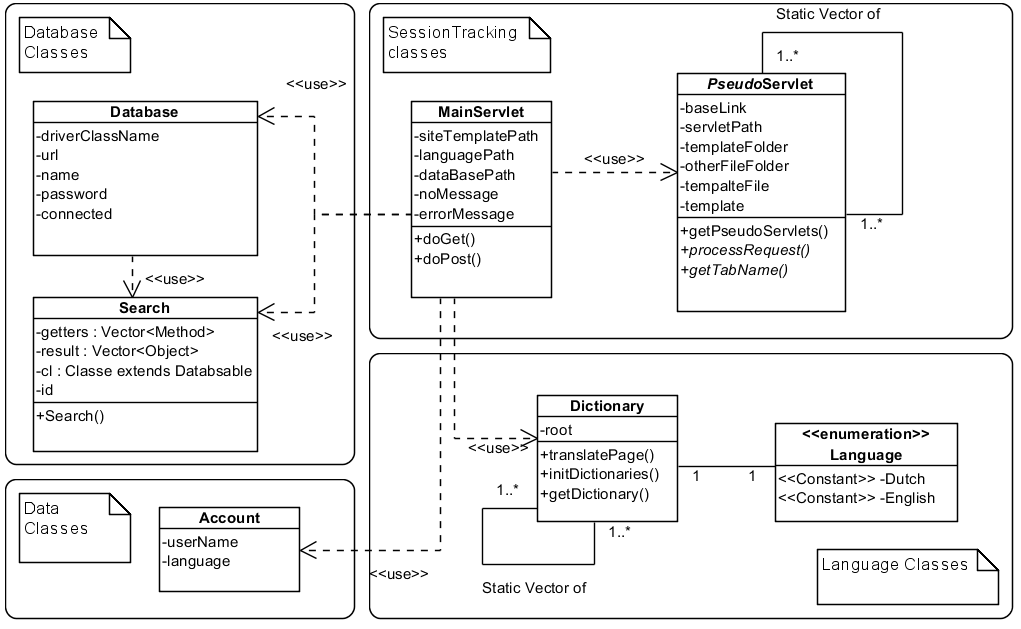
\includegraphics[width=\columnwidth]{UML_MainServlet_Dependencies.PNG}%
\end{figure}

\newpage

%-----------------------------------------------------------------------------------------------------------------------------------------------------------------

\section{Session Tracking}

\subsection{Overzicht}

Als een gebruiker zich succesvol aanmeldt op de website zal de mainServlet voor hem een session aangemaakt die zijn account bevat. Elke session heeft een uniek ID wat de mainServlet toelaat bestaande sessions op te zoeken in een algemene tabel. Telkens de gebruiker een get of post request doet, moet hierbij zijn session id worden meegegeven. Om dit te bereiken wordt aan  alle URLs het sessionID van de gebruiker toegevoegd. Op deze mannier kan de mainServlet voor elke request nagaan welke session er bij de gebruiker hoort. 

\subsubsection{UMLDiagrammen}
\begin{figure}%
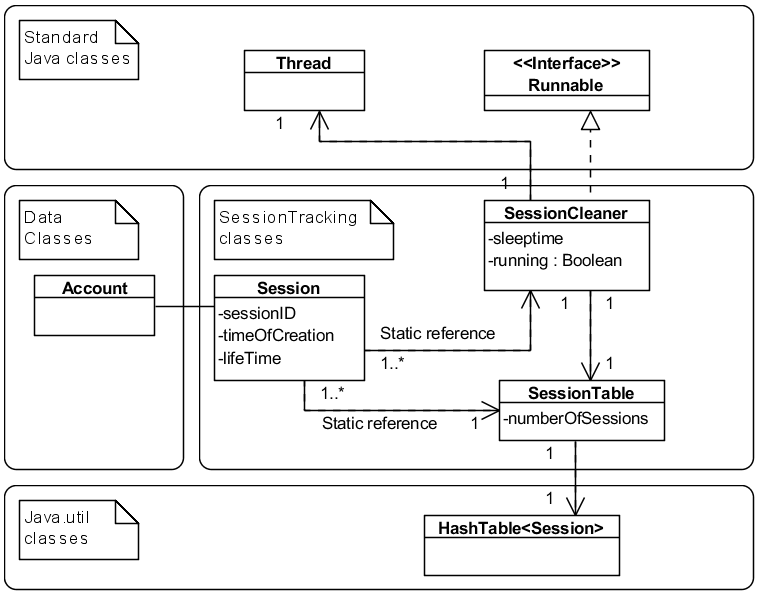
\includegraphics[width=\columnwidth]{UML_SessionTracking.PNG}%
\end{figure}

\subsubsection{Klassen}

\subsubsubsection{Session}
Klasse die een websessie voorstelt.\\

Telkens een gebruiker zich succesvol aanmeldt moet de MainServlet een session cre�ren. Deze bevat zowel de accountgegevens van de gebruiker als een sessionID. Elke session die wordt aangemaakt wordt automatisch opgeslagen in een statische sessionTable die vervat zit in de Session klasse. Sessies die aanwezig zijn in deze algemene tabel kunnen worden opgevaagt via de methode getSession.\\
Een session is slecht geldig voor een vooraf bepaalde tijd die men de levenstijd noemt. Als de gebruiker gedurende een volledige levenstijd inactief is gebleven of hij meldt zich af  dan wordt de sessie niet langer als geldig bevonden. Dit heeft als resultaat dat de gebruiker weer naar het login scherm wordt verwezen. Om vervallen sessions automatisch uit de algemene tabel te verwijderen bevat de Session klasse ook een sessionCleaner. Dit laat toe om sessions van gebruikers die zich niet hebben afgemeld maar toch de site hebben verlaten ook te verwijderen uit de tabel.

\subsubsubsection{SessionTable}
Klasse die wordt gebruikt om session in op te slaan.\\

De sessionTable omsluit een hashTable. Als key van de hashTable wordt het sessionID gebruikt.  Als veld wordt een session zelf meegegeven. Het is ook mogelijk om het aantal element in de sessionTabel op te vragen. 

\subsubsubsection{SessionCleaner}
Klasse die gebruikt wordt om vervallen sessions automatische te verwijderen.\\

De klasse SessionCleaner implementeert de interface runnable. Dit laat toe om een thread op te starten waarin de run methode van de klasse wordt uitgevoerd. Een sessionCleaner bevat steeds zelf een thread die zijn run methode uit voerd. Het is dus niet nodig om deze extern aan te maken. Tijdens de thread wordt in de toegekende sessionTable sequentieel gezocht naar vervallen sessions. Hierbij is het belangrijk dat de toegewezen tabel op een gesynchroniseerde mannier wordt gewijzigd. 

\newpage

\section{Language Resolving}

\subsection{Overzicht}
Om het mogelijk te maken aan de gebruiker om de taal van de site aan zijn voorkeur te kunnen aanpassen werd een klassenstructuur ontwikkeld die bepaalde stukken tekst  op de webpagina's vervangt volgens de overeenkomstige taal. 

\subsubsection{UMLDiagrammen}
\begin{figure}%
\includegraphics[width=\columnwidth]{UML_languageClasses.PNG}%
\end{figure}

\subsubsection{Klassen}

\subsubsubsection{LanguageTag}
Klasse die een vertaalbaar stuk tekst voorstelt.\\

Een languageTag is een string die moet worden vervangen door de languageResolver en wordt gebruikt als een sleutel in een woordenboek. Het format van een languageTag ligt vast en zal worden gecontroleerd als de languageTag wordt gemaakt of gewijzigd. Als het format niet overeenkomt met het verwachte format wordt een DataFormatException gegenereerd. Het huidige format is ##tagname##.

\subsubsubsection{Dictionary}
Klasse die een hashtable omvat met LanguageTags als sleutel en Strings	als waarde\\

Een dictionay wordt gebruikt door de LanguageResolver om LanguageTags te vertalen naar een specifieke taal. Normaal worden Dicitonarys gemaakt aan de hand van taalfbestanden. Deze worden gekenmerkt door de .l extensie. Invoer in een taalbestand moeten van de volgende vorm zijn  ##languageTag##=value; De taal gekoppeld aan het woordenboek zal het zelfde zijn als de naam van het taalbestand (zonder de extensie).

\subsubsubsection{LanguageResolver}
Een statische klasse die gebruikt wordt door de MainServlet om LanguageTags op te lossen \\

De LanguageResolver vertaalt tekst naar een gegeven taal. Dit houdt in dat hij alle LanguageTags in de tekst vervangt door hun overeenkomstige waarde. Hiervoor maakt hij gebruik van een set van Dicitonarys. Deze worden geladen tijdens het maken van het klasse object

\newpage


%-----------------------------------------------------------------------------------------------------------------------------------------------------------------

\section{Algoritme voor kalenderplanning}

\subsection{Inleiding}

Het doel is om op basis van informatie uit de Database een lessenrooster op te stellen dat aan bepaalde vereisten voldoet. Deze informatie zal via een webinterface kunnen worden ingevoerd door daartoe bevoegde personen. De lessenroosters zullen per semester worden opgesteld. Dit gebeurt in door een object van een klasse die SemesterScheduler heet. Dit object zal dan per semester CalendarFiles genereren die het lessenrooster beschrijven en deze zullen dan worden opgeslagen in de Database.

\subsection{Overzicht van de klasse SemesterScheduler}

\subsubsection{Variabelen:}

\begin{itemize}
	\item[] Vector$<$Educator$>$ educators  (lijst van de docenten) 
	\item[] Vector$<$Program$>$ programs  (lijst van de programma�s: bv. 1 Ma EIT) 
	\item[] Vector$<$Room$>$ rooms  (lijst van de lokalen) 
	\item[] Vector$<$Course$>$ courses  (lijst van de vakken die moeten ingedeeld worden) 
\end{itemize}

Bovenstaande vectoren bevatten variabelen uit het package DataStructure, deze klassen bevatten de informatie die nodig is om het lessenrooster op te stellen. Ze zullen uit de Database worden ingeladen met de methode loadData().

\begin{itemize}
	\item[] int numberOfweeks
	\item[] int startingHour
	\item[] int endingHour
\end{itemize}

Deze drie integers bepalen enkele tijdsdimensies van het lessenrooster. numberOfWeeks bepaalt het aantal weken van de semester. startingHour en endingHour resp. het begin- en einduur per dag (bv. van 8 tot 18 uur)

\begin{itemize}
	\item[] Hashtable$<$Educator,Vector$<$Integer$>>$ unavailableHoursForEducator 
	\item[] Hashtable$<$Program,Vector$<$Integer$>>$ unavailableHoursForProgram 
\end{itemize}

Deze  hashing tables zullen bijhouden welke uren er niet meer beschikbaar zijn voor een programma of een docent. Dit om dubbelboekingen te bekomen. Voor de docenten bestaat de mogelijkheid om via de webinterface data in te geven waarop hij of zij niet beschikbaar is. (Zie ook verder bij de klasse Constraint.)

\subsubsection{Methodes:}
\begin{itemize}
	\item[] \textit{SemesterScheduler(int startingHour, int endingHour, int numberOfweeks)}  \\
	De constructor waaraan de tijdsvariabelen worden meegegeven.
	\item[]\textit{solve()} \\
	Deze methode zal het lessenrooster voor heel de semester opstellen en dan de bekomen CalendarFiles wegschrijven in de Database.
\end{itemize}

De lijst van onderstaande methoden zullen verder in dit document worden aangehaald en dan daar worden uitgelegd.
\begin{itemize}
	\item[] generateCalendars() 
	\item[] loadData() 
	\item[] createBlocks() 
	\item[] initializeUnavailableHours(...) 
	\item[] calcNextNewSpace(...) 
	\item[] addUnavailableBlock(...) 
	\item[] removeUnavailableBlock(...) 
	\item[] makeWeekSchedule(...)
\end{itemize}

\subsection{De solver (methode solve() )}

Deze methode zal uiteindelijk alle methoden bevatten die ervoor zorgen dat er een lessenrooster wordt opgesteld. In de constructor is de nodige data reeds ingeladen a.d.h.v. de methode \textit{loadData()}. 

De bedoeling is dat er nu per week een lessenrooster wordt opgesteld. Hiervoor is het dus nodig dat de data over het aantal weken worden verdeeld. Het algoritme dat het rooster per week opstelt is een backtrackingalgoritme. 

De vector courses bevat alle vakken die moet ingedeeld worden per semester. De klasse course bevat echter nog eens een vector met daarin de klasse Subcourse. Deze klasse geeft aan over welk type les (hoorcollege, werkcollege, labo,...) gaat en bevat ook hoeveel uren er van dit type zijn en hoe lang een minimum blok moet zijn. Per Subcourse zullen er dan object van de klasse Subcourseblock gegenereerd worden. Deze klasse heeft een verwijzing naar zijn Subcourse en bevat de lengte van het blok. Deze blocks moeten dan over het lessenrooster verdeeld worden. Deze blocks moeten echter ook nog eens per week ingedeeld worden. Daarom heeft elk object van Subcourse een veld met daarin een beginweek (geeft aan wanneer deze lessen beginnen) en een minimum aantal uur per week. Er zal hiervoor een methode worden opgeroepen die \textit{createBlocks()} heet. Deze geeft een Vector$<$Vector$<$Subcourseblock$>>$ terug. Dit interpreteert men als volgt: elke week heeft een vector van Subcourseblocks. De index van de buitenste vector geeft de week aan. \\

Vector$<$Course$> \rightarrow$ Vector$<$Subcourse$> \rightarrow$ Vector$<$Vector$<$Subcourseblock$>>$ \\

De methode \textit{createBlocks()} roept een methode op uit de klasse Subcourseblock; \textit{generateBlocksPerWeek(Vector$<$Course$>$ courses, int NumberOfWeeks)}.

\subsubsection{Pseudocode generateBlocksPerWeek}

\begin{verbatim}
weeks =  new Vector<Vector<Subcourseblock>>
Maak voor elke week een Vector<Subcourseblock> (for lus)
  Vraag voor elke Course zijn Subcourses op. (for lus1)
    Ga elke Subcourse af. (for lus2)
      Genereer zijn Subcourseblocks (while lus)
		
        Verdeel ze over de weken a.d.h.v. zijn beginweek 
        en minimum aantal uur per week.
        Voeg de Subcourseblock toe bij de juiste week
		
      End (while lus)
    End (for lus2)
  End (for lus1)
End (for lus)  
Return weeks
\end{verbatim}

Vervolgens zal in \textit{solve()} voor elke week de daarbij horende vector van Subcourseblocks worden de methode \textit{makeWeekSchedule(Vector$<$Subcourseblock$>$ blocks, Vector$<$Room$>$ rooms, int numberOfDays)} opgeroepen. Deze methode zal dan het backtrackingalgoritme uitvoeren en de bekomen resultaten omzetten in calendarfiles. (Meer over deze methode in de volgende paragraaf.)

\subsubsection{Pseudocode solve}

\begin{verbatim}
Maak de Subcourseblocks en verdeel ze over de weken.

(Vector<Vector<Subcourseblock>>  weeks  = createBlocks())

Ga de vector weeks af en haal er per week de blocks uit. 
Los dan vervolgens het probleem op per week. (for lus)

    Vector<Subcourseblock> = blocks
    makeWeekSchedule(...)

End (for lus)
\end{verbatim}


\subsection{Het backtrackingalgoritme per week (methode makeWeekSchedule)}

Deze methode zal een vector van Subcourseblocks invullen in lessenrooster. Men geeft de vector mee. Bovendien geeft men ook een vector mee met daarin het aantal beschikbare lokalen. Men geeft ook mee over hoeveel dagen het lessenrooster gespreid is.

\subsubsection{De SpaceTimeMatrix: }

De methode beschikt reeds over een lijst van blocks die moeten ingedeeld worden in het lessenrooster. Het lessenrooster zelf is echt nog niet voorgesteld. Om dit te doen bestaat er een klasse die SpaceTimeMatrix heeft. Deze klasse zal variabelen bevatten die de tijd-ruimte structuur van het rooster voorstellen, alsook methoden voor een geplaatste Subcourseblock het uur, de dag en het lokaal in de week teruggegeven. De belangrijktse variabele van deze klasse is de array Matrix met daarin booleans. De booleans geven weer of de plaats in het lessenrooster al dan niet is ingenomen (true == nog vrij, false == reeds ingenomen). De index van de array stelt de tijd-ruimte structuur voor. 

Dit gebeurt als volgt:

\begin{figure}%
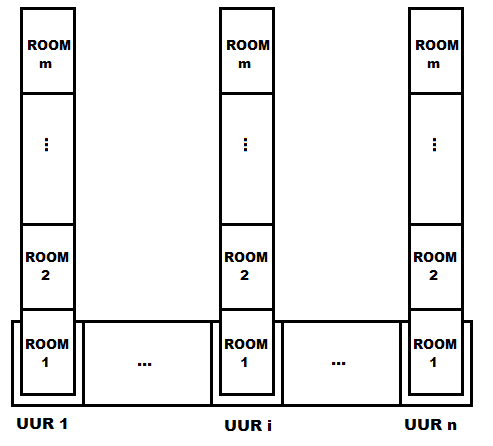
\includegraphics[width=\columnwidth]{spacetime.png}%
\caption{De SpaceTimeMatrix}%
\end{figure}

\begin{itemize}
	\item[] Hour loopt van 1 tot (numberOfDays*(endingHour-startingHour)-1):  bv. 0 tot 39 (Dit stelt dan 40 uur voor. 5 werkdage en elke dag 8 uur) 
	\item[] numberOfRooms is het aantal lokalen (rooms.size() ) 
	\item[] roomNumber is de index van de room in rooms. 
	\item[] index = hour * numberOfRooms + roomNumber (1) 
	\item[] Uit (1) haalt men dan de informatie voor het lessenrooster als volgt: 
	\item[] roomNumber = index mod numberOfRooms 
	\item[] hour = (index � (index mod numberOfRooms)) / numberOfRooms 
	\item[] hourInDay = hour mod (endingHour-startingHour) (bv. 4e uur van een dag) 
	\item[] Day = (hour � hourInDay) / (endingHour-startingHour)
\end{itemize}

Deze klasse stelt dan het eigenlijke lessenrooster voor. Per Subcourseblock zullen dan de indices worden opgeslagen van de toegekende plaatsen en hieruit haalt men dan de tijdsinformatie.

Overzicht van de klasse SpaceTimeMatrix
\begin{itemize}
	\item[] \textbf{Variabelen:} 
\item[] \begin{itemize}
	\item[] \textit{Boolean[] Matrix}
	\item[] \textit{int startingHour}
	\item[] \textit{int endingHour}
	\item[] \textit{int numberOfDays}
	\item[] \textit{int numberOfRooms}
\end{itemize}
\item[] \textbf{Methoden:} \\
\item[]
\begin{itemize}
	\item[] \begin{itemize}
	\item[] \textit{SpaceTimeMatrix(int startingHour, int endingHour, int numberOfDays, int numberOfRooms)} 
\end{itemize}
	\item[] Methoden om dingen op te vragen of aan te passen in de SpaceTimeMatrix
	\item[] \begin{itemize}
		\item[] \textit{changeBlockAt(int i, Boolean b, int blocksize)}
		\item[] \textit{checkBlockAt(int i, Boolean b, int blocksize)}
		\item[] \textit{isWithinRange(int i)} 
	\end{itemize}
	\item[] Methoden om de indices om te zetten.
	\item[] \begin{itemize}
		\item[] \textit{giveHour(int i)}
		\item[] \textit{giveRoom(int i)}
		\item[]\textit{ giveHourInDay(int i)}
		\item[] \textit{giveDay(int i) }
\end{itemize}
	
\end{itemize}
\end{itemize}

\subsubsection{Het algoritme:}

Het algoritme om een weeklessenrooster is pure backtracking. Om dit op een effici�nte manier te kunnen verwezenlijken heeft men de klasse Node ontwikkeld. Deze klasse bevat de toegekende Subcourseblock, de plaats in het lessenrooster (m.a.w. de index in de SpaceTimeMatrix) en een verwijzing naar de vorig toegekende Node. Aan de hand van deze verwijzing kan men dan teruggaan naar een vorige stap, als men op een doodlopend spoor terecht komt.

Het algoritme zal een vector van Subcourseblocks afgaan en dan steeds een plaats zoeken voor elke Subcourseblock in het lessenrooster; deze gegevens dan in een Node steken en dan naar de volgende Subcourseblock overgaan. Om een plaats te zoeken scant men de SpaceTimeMatrix af en gaat men telkens na of een bepaalde plaats voor die Subcourseblock in aanmerking komt. Om na te gaan of een bepaalde plaats in aanmerking komt, moet men de vereisten voor het lessenrooster nagaan. Deze vereisten worden in de onderstaande kader weergegeven.

Vereisten waaraan het rooster moet voldoen: 
\begin{itemize}
	\item[(1)] Er mag geen dubbelboeking van een lokaal optreden. 
	\item[(2)] Het lokaal moet groot genoeg zijn voor het aantal studenten. 
	\item[(3)] Het lokaal moet het nodige materiaal voor een les bevatten. 
	\item[(4)] Programma�s mogen niet dubbel geboekt zijn.
	\item[(5)] Een docent mag niet dubbelgeboekt zijn.
	\item[(6)] Een docent moet beschikbaar zijn.
	\item[(7)] Op vakantiedagen mag er niets gepland zijn.
\end{itemize}

Om deze vereisten na te kunnen gaan, als men een Subcourseblock in een het lessenrooster wilt plaatsen, heeft men de klasse Constraint gecre�erd. Deze klasse is een verzameling van staticsche methodes die steeds een Boolean terug gegeven om aan te geven of er al dan niet aan de vereisten voldaan is (false indien niet, true indien wel).

Overzicht van de klasse Constraint
\begin{itemize}
	\item[] \textit{int i} \\
	Dit is de index in de SpaceTimeMatrix die men evalueert. Hieruit kan men alle nodige informatie afleiden (zie ook SpaceTimeMatrix).
	\item[] \textit{roomAvailableAtBlock(int i, Room room, Subcourseblock block)}
	Deze methode checkt of het lokaal gedurende periode van het Subcourseblock nog beschikbaar is. (1)
	\item[] \textit{roomSufficient(int i, Room room, Subcourseblock block)} \\
	Deze methode checkt of het lokaal groot genoeg is en het vereiste materiaal bevat. (2) en (3)
	\item[] \textit{hourAvailable(int i, Subcourseblock block, Hashtable hoursAvailableForEducator, Hashtable hoursAvailableForProgram)}
	Deze methode gaat na of er geen dubbelboekingen zijn voor de docent of voor het programma. hoursAvailableForEducator en hoursAvailableForProgram zijn objecten van de klasse Hashtable (hashingtables) waarin de vectoren zijn opgeslagen met daarin de reeds toegekende uren voor een docent of voor een programma. (4) en (5) 
\item[] \textit{dateAvailable(int i, Subcourseblock block)} \\
Deze methode gaat na of de dag waarop men iets wilt zetten geen verlofdag is en of de docent op die dag wel beschikbaar is. Dit gebeurt aan de hand van Calendarfiles. Elke docent heeft een persoonlijke Calendarfile en er is een algemene Calendarfile met daarin de verlofdagen voor een semester. Deze methode gaat overlappingen na. Indien er een overlapping is, is er niet aan deze vereiste voldaan. (6) en (7)
\end{itemize}
Tijdens het backtracken, zal er steeds vooraleer men een Subcourseblock kan plaatsen de methode calcNext(int i) worden opgeroepen. Deze methode zal steeds de volgende beschikbare plek in het lessenrooster teruggegeven. Ze gaat de indices van de SpaceTimeMatrix af en de eerst mogelijke die voldoet aan de vereisten wordt teruggegeven. De index die men meegeeft is de laatst toegekende plek in het rooster.

\subsubsection{Het backtrack algoritme:}

\begin{verbatim}
Zolang niet elke block is toegekend (while lus)

Zoek een plek in het rooster

    Plek gevonden: 
    Vul deze plek in SpaceTimeMatrix
    Maak een Node aan
    Zorg dat de uren voor de docent en het programma onbeschikbaar zijn

End (while lus)
\end{verbatim}

Aan elke Subcourseblock zal zijn plaats de SpaceTimeMatrix worden toegekend. Aan de hand van deze	informatie zal hij dan de dag, het uur in die dag en het lokaal kennen. Zijn week kent hij ook. Op die manier zal elke Subcourseblock alle informatie bevatten om in een Calendarfile te plaatsen.

\subsection{Het aanmaken van Calendarfile (getCalendar() )}

Elke Subcourseblock heeft nu een plek in het rooster. Nu moet dit nog omgezet worden in een bruikbare structuur die door gebruikers kan worden geraadpleegd. Hiervoor zal men per Subcourse een Calendarfile maken. De som van al deze Calendarfiles zal dan het hele lessenrooster voor de hele universiteit zijn. 

De methode \textit{getCalendar()} zal alle Subcourseblocks afscannen en dan steeds hun Subcourse opvragen. Hiervan vraagt men dan de Calendarfile op en het Subcourseblock zal dan hieraan worden toegekend.

% Matthias schrijft dit wel
%\subsection{Design concerns}
%
%Het algoritme dient in staat te zijn om een lessenrooster te maken dat aan bepaalde voorwaarden (constraints) voldoet. Het is daarom belangrijk dat deze eerst bepaald worden. Men kan een indeling maken in deze voorwaarden. Zo zijn er de \textit{fixed} constraints aan deze moeten zeker voldaan zijn, anders klopt het lessen rooster niet. \textit{Hard constraints} deze moeten zo goed mogelijk vervuld zijn en dan zijn er nog \textit{soft constraints} deze staan onderaan de ladder en hoeven dus niet noodzakelijk vervuld te zijn. Aan de hand van deze voorwaarden kan men dan nagaan hoe goed het lessenrooster is. Dit doet men aan de hand van een \textit{fitnessvalue}. Zo krijgt een geplaatste les 3 punten als aan een \textit{fixed constraint} voldaan is, 2 voor een hard en 1 voor een soft. Aangezien de \textit{fixed constraints} zeker voldaan moeten zijn, moet een geplaatste les al zeker 12 punten hebben. Op die manier kan men het resultaat evalueren.
%
%\begin{itemize}
%\item[] \textit{Fixed constraints}\\[-3mm]
%\begin{enumerate}
%	\item Er mag nooit meer dan 1 les gepland zijn in een leslokaal \\[-3mm]
%	\item Een docent (educator) kan niet meer dan 1 les geven  \\[-3mm]
%	\item Een leslokaal (room) moet groot genoeg zijn voor het aantal studenten \\[-3mm]
%	\item Als een les bepaald materiaal vereist (zoals computer, laboratorium,...) moet hier aan worden tegemoet gekomen. \\[-3mm]
%\end{enumerate}
%\item[] \textit{Hard constraints} \\[-3mm]
%\begin{enumerate}
% \item Het lessenrooster van een student mag niet overlappen. \\[-3mm]
% \item Er mag van een vak bijvoorbeeld hoogstens 4 uur per dag gegeven worden. \\[-3mm]
% \item Student mogen bijvoorbeeld maximum 8 uur les per dag krijgen. \\[-3mm]
%\end{enumerate}
%\item[] \textit{Soft constraints} \\[-3mm]
%\begin{enumerate}
% \item De werkcolleges mogen pas na of gelijktijdig met de theoriecolleges beginnen. \\[-3mm]
%\end{enumerate}
%\end{itemize}
%
%Voor iedere week van het academisch jaar zal de lessenrooster een tabel bevatten voor elke student die bestaat uit 5 dagen (maandag t.e.m. vrijdag) waar voor elke dag de uren bijstaan (er kan les gegeven worden van 8u t.e.m. 18u). \\
%
%Het algoritme zal deze tabel in een eerste fase zo opbouwen dat er aan de fixed constraints voldaan is en dan in een tweede fase proberen om de totale fitnessvalue op te drijven.
%
%\subsection{Design elements}
%
%Om het algoritme te kunnen uitvoeren is er natuurlijk de nodige informatie nodig om tot een lessenrooster te kunnen komen. De informatie die nodig is, zal uit een database worden gehaald en dan in klassenstructuur gegoten worden. Deze klassenstructuur is besproken in "Design Viewpoint 2: Logical".
%Het schema en bijbehorende uitleg kan daar gevonden worden.
%Deze structuur zal nog worden uitgebreid met methode die de rooster opstellen en dan hieruit vertrekkende de fitnessvalue bepalen. De bovenstaande structuur zal met andere woorden nog worden uitgebreid.

%\section{Design rationale}


%\begin{figure}
%\begin{center}
%\includegraphics[width=\textwidth]{Bangladesh}
%\caption*{Bangladesh}
%\end{center}
%\end{figure}

%\begin{tabular}[t]{llll}
%Mandi & Katholiek & 25\% & Platte neus -- spleetogen \\
%Gohli & Moslims   & 75\% & Grote ogen -- scherpere neus \\
%Kooch & Hindu     & 1\%  & Mengeling van de twee \\
%\end{tabular}
%\\[5mm]

%\begin{itemize}
%\item[.] Slaapmatje \\[-3mm]
%\item[.] Kleren: 3 korte broeken, 6 onderbroeken, 4 T-shirts\\[-3mm]
%\item[.] Longi: voor 's avonds en als pyjama\\[-3mm]
%\item[.] Tandenborstel en twee tubes tandpasta\\[-3mm]
%\end{itemize}


 \end{document}